\section{Representação de sistemas discretos em espaço de estados}

\begin{frame}{Introdução}
\begin{block}{Motivação}
	\begin{itemize}
		\item Considere a seguinte equação de diferenças:
	\end{itemize}
$$y(k) = -y(k-1) + u(k) -u(k-1)$$
\vspace{-0.3cm}
	\begin{itemize}
		\item A ordem de um sistema dinâmico é dada pelo maior atraso na variável de saída, que neste caso, é igual a 1; embora este diagrama utilize \textbf{duas posições de memória} (\textit{representado pelo operador atraso $q^{-1}$}).
		\item Tomando a transformada $\mathcal{Z}$ da equação de diferenças, temos:
	\end{itemize}
$$Y(z) = -Y(z)z^{-1} + U(z) - U(z)z^{-1} \implies \dfrac{Y(z)}{U(z)} = \dfrac{1-z^{-1}}{1+z^{-1} } = \dfrac{z-1}{z+1}$$
\end{block}
\centerline{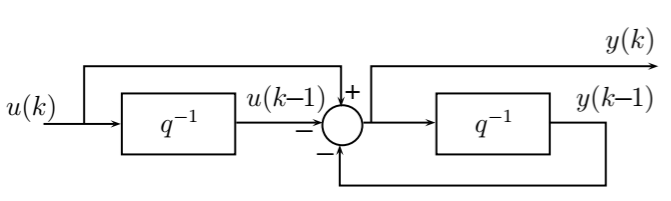
\includegraphics[width=0.65\linewidth]{Figuras/Ch14/fig1.PNG}}
\end{frame}

\begin{frame}{Introdução}
\begin{block}{Motivação}
	\begin{itemize}
		\item Considere agora as seguintes equações de diferenças:
	\end{itemize}
$$x(k) = u(k) -x(k-1) \quad \text{e} \quad y(k) = x(k) - x(k-1)$$
\vspace{-0.3cm}
	\begin{itemize}
		\item Tomando a transformada $\mathcal{Z}$ das equações de diferenças, temos:
	\end{itemize}
$$X(z) = U(z) - X(z)z^{-1} \implies X(z) = \dfrac{U(z)}{1+z^{-1}}$$
$$Y(z) = X(z) - X(z)z^{-1} \implies Y(z) = \dfrac{U(z)}{1+z^{-1}}{(1-z^{-1})} \implies \dfrac{Y(z)}{U(z)} = \dfrac{z-1}{z+1}$$
\end{block}
\vspace{0.2cm}
\centerline{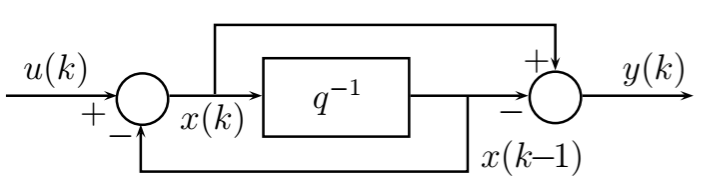
\includegraphics[width=0.6\linewidth]{Figuras/Ch14/fig2.PNG}}
\end{frame}

\begin{frame}{Introdução}
\begin{block}{Motivação}
	\begin{itemize}
		\item Apesar de os sistemas possuírem representações diferentes, a \textbf{função de transferência em ambos é igual}.
		\item No segundo sistema, o operador de atraso não atua sobre os sinais de  entrada e saída, mas o faz sobre uma \textbf{variável interna ao sistema}, $x(k)$. Esta variável é conhecida como \textbf{variável de estado} (\textit{definida no domínio do tempo discreto}).
	\end{itemize}
\end{block}
\end{frame}

\begin{frame}{Estado de um sistema}
\begin{block}{Definição}
	\begin{itemize}
		\item O estado do sistema é representado pelo vetor de estado $\bm{x}(k) \in \mathbb{R}^n$.
		\item Geometricamente, $\bm{x}(k)$ corresponde a um \textbf{ponto no espaço Euclidiano} de dimensão $n$ no instante $k$. À medida que $k$ aumenta, esse ponto pode mover-se no espaço, representando uma mudança no estado  do sistema.
		\item O vetor de estado é composto pelo \textbf{menor número de variáveis necessárias} ($n$) para determinar unicamente o estado do sistema.
	\end{itemize}
\end{block}
\centerline{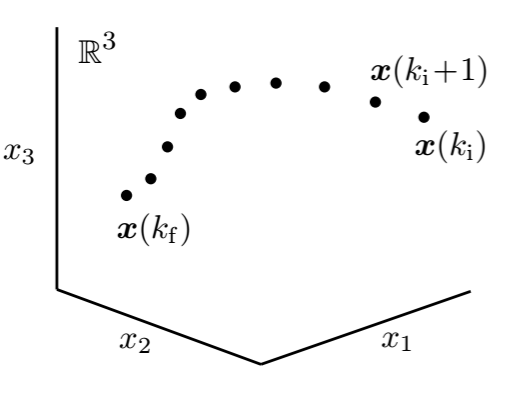
\includegraphics[width=0.4\linewidth]{Figuras/Ch14/fig3.PNG}}
\end{frame}

\begin{frame}{Espaço de estados}
\begin{block}{Representação de um SLIT em espaço de estados}
	\begin{itemize}
		\item Considerando um Sistema Linear e Invariante no Tempo (SLIT), a \textbf{representação em espaço de estados} é dada por:
	\end{itemize}
\begin{align*}
    \bm{x}(k+1) &= A\bm{x}(k) + B\bm{u}(k) \qquad \text{\textit{equação dinâmica}} \\
    \bm{y}(k) &= C\bm{x}(k) + D\bm{u}(k) \qquad \text{\textit{equação de saída}}
\end{align*}
\vspace{-0.3cm}
	\begin{itemize}
		\item[] onde $\bm{x} \in \mathbb{R}^n$ é o \textbf{vetor de estado}, $\bm{u} \in \mathbb{R}^r$ é o \textbf{vetor de entradas} e $\bm{y} \in \mathbb{R}^p$ é o vetor de saídas. Além disso, $A \in \mathbb{R}^{n \times n}$, $B \in \mathbb{R}^{n \times r}$, $C \in \mathbb{R}^{p \times n}$ e $D \in \mathbb{R}^{p \times r}$.
		\item \textbf{A representação em espaço de estados não é única}, ou seja, um mesmo sistema pode ser representado por vetores de estado distintos, o que resultará em um \textbf{diferente conjunto de  matrizes} ($A, B, C, D$).
		\item Vantagens na representação em espaço de estados:
	    \begin{enumerate}
	        \item É mais adequada para lidar com sistemas \textbf{multivariáveis}.		\item É possível representar sistemas \textbf{não lineares} em espaço de estados.
	    \end{enumerate}
	\end{itemize}
\end{block}
\end{frame}

\begin{frame}{Equação característica}
\begin{block}{Definição}
	\begin{itemize}
		\item Considere
	\end{itemize}
$$A \bm{v} = \lambda \bm{v}$$
\vspace{-0.3cm}
	\begin{itemize}
		\item[] onde $A \in \mathbb{R}^{n \times n}$, $\bm{v} \in \mathbb{C}^{n}$ é um vetor não nulo e $\lambda \in \mathbb{C}$ é um escalar.
		\item Com isso,
	\end{itemize}
$$0 = (\lambda I - A) \bm{v}$$
\vspace{-0.3cm}
	\begin{itemize}
		\item Para que a equação tenha solução não trivial ($\bm{v} \neq 0$) é necessário que
	\end{itemize}
$$\boxed{|\lambda I - A| =  0} \qquad \text{\textit{equação característica}}$$
\vspace{-0.3cm}
    \begin{itemize}
		\item Os valores de $\lambda_i$, $i = 1, 2, ..., n$ são os \textbf{autovalores} da matriz $A$.
		\item Os respectivos $\bm{v}_i$, $i = 1, 2, ..., n$ são os \textbf{autovetores} da matriz $A$.
	\end{itemize}
\end{block}
\end{frame}

\begin{frame}{Equação característica - Exemplo \#01}
\begin{block}{Problema}
Considere o sistema discreto:

\begin{align*}
    \begin{bmatrix} x_1(k+1) \\ x_2(k+1) \end{bmatrix}
    &=
    \begin{bmatrix}
    0 & 1 \\ -\num{0,2} & \num{1,2}
    \end{bmatrix}
    \begin{bmatrix}
    x_1(k) \\ x_2(k)
    \end{bmatrix}
    +
    \begin{bmatrix}
    0 \\ 1
    \end{bmatrix}
    u(k) \\
    y(k)
    &=
    \begin{bmatrix}
    5 & -25
    \end{bmatrix}
    \begin{bmatrix}
    x_1(k) \\ x_2(k)
    \end{bmatrix}
\end{align*}
Determine os autovalores de $A$.
\end{block}
\end{frame}

\begin{frame}{Equação característica - Exemplo \#01}
\begin{block}{Resolução}
\begin{itemize}
    \item A equação característica pode ser escrita como:
\end{itemize}

\begin{align*}
    \Delta(\lambda) &= |\lambda I - A| =  0 \\
    &= \Bigg|\lambda \begin{bmatrix}
    1 & 0 \\ 0 & 1 \end{bmatrix} - \begin{bmatrix}
    0 & 1 \\ -\num{0,2} & \num{1,2}
    \end{bmatrix}\Bigg| = 0 \\
    &= \Bigg|\begin{bmatrix}
    \lambda & -\num{1} \\ \num{0,2} & \lambda-\num{1,2} \end{bmatrix}\Bigg| = 0 \\
    &= \lambda^2 -\num{1,2}\lambda + \num{0,2} = 0
\end{align*}
\begin{itemize}
    \item Lembrando que os valores de $\lambda_i$ são os autovalores da matriz $A$, temos:
\end{itemize}
$$\lambda_1 = 1 \qquad \lambda_2 = \num{0,2}$$
\end{block}
\end{frame}

\begin{frame}{Formas canônicas}
\begin{block}{Introdução}
\begin{itemize}
    \item Podemos utilizar as formas canônicas para encontrar a representação em espaço de estado para uma dada função de transferência.
    \item As formas canônicas que serão estudadas são:
    \begin{enumerate}
        \item Forma canônica controlável;
        \item Forma canônica observável;
        \item Forma canônica de Jordan.
    \end{enumerate}
    \item Por simplificação, iremos considerar sistemas SISO (\textit{Single Input Single Output}), isto é, apenas uma entrada e uma saída.
    \item Em todos os casos, considere que o sistema discreto possua a seguinte função de transferência:
\end{itemize}
$$G(z) = \dfrac{Y(z)}{U(z)} = \dfrac{b_{n-1}z^{n-1}+b_{n-2}z^{n-2} + \cdots + b_1z+b_0}{z^n+a_{n-1}z^{n-1}+ \cdots + a_1z+a_0}$$
\end{block}
\end{frame}

\begin{frame}{Forma canônica controlável}
\begin{block}{Representação}
\begin{itemize}
    \item A \textbf{forma canônica controlável} de $G(z)$ é representada como:
\end{itemize}

\begin{align*}
    \begin{bmatrix} x_1(k+1) \\ x_2(k+1) \\ \vdots \\  x_{n-1}(k+1) \\ x_n(k+1) \end{bmatrix}
    &=
    \begin{bmatrix}
    0 & 1 & 0 & \cdots & 0 \\
    0 & 0 & 1 & \cdots & 0 \\
    \vdots & \vdots & \vdots & \ddots & \vdots \\
    0 & 0 & 0 & \cdots & 1 \\
    -a_0 & -a_1 & -a_2 & \cdots & -a_{n-1}
    \end{bmatrix}
    \begin{bmatrix} x_1(k) \\ x_2(k) \\ \vdots \\  x_{n-1}(k) \\ x_n(k) \end{bmatrix}
    +
    \begin{bmatrix}
    0 \\ 0 \\ \vdots \\ 0 \\ 1
    \end{bmatrix}
    u(k) \\
    y(k)
    &=
    \begin{bmatrix}
    b_0 & b_1 & \cdots & b_{n-2} & b_{n-1}
    \end{bmatrix}
    \begin{bmatrix}
    x_1(k) \\ x_2(k) \\ \vdots \\  x_{n-1}(k) \\ x_n(k)
    \end{bmatrix}
\end{align*}
\end{block}
\end{frame}

\begin{frame}{Forma canônica controlável}
\begin{block}{Comentários}
\begin{itemize}
    \item A forma canônica controlável é uma \textbf{realização} (\textit{implementação}) da função de transferência $G(z)$.
    \item Dada uma função de transferência $G(z)$, a forma canônica controlável pode ser obtida por \textbf{inspeção}.
    \item Além disso, \textbf{a entrada afeta todos os estados} independentemente dos valores dos parâmetros $a_i$ e $b_j$ (\textit{o que justifica o ``controlável"}).
\end{itemize}
\end{block}
\end{frame}

\begin{frame}{Forma canônica controlável}
\begin{block}{Comentários}
\begin{itemize}
    \item As variáveis de estado são as saídas dos blocos com o operador de atraso $q^{-1}$ no \textbf{diagrama de simulação}. 
\end{itemize}
\end{block}
\centerline{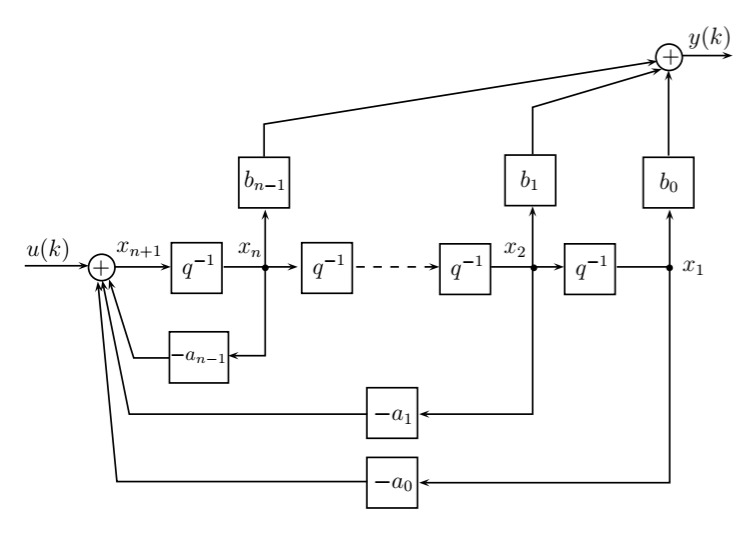
\includegraphics[width=0.73\linewidth]{Figuras/Ch14/fig4.PNG}}
\end{frame}

\begin{frame}{Forma canônica controlável}
\begin{block}{Comentários}
\begin{itemize}
    \item As variáveis de estado aparecem nos nós que seguem ramos com ganho $z^{-1}$ no \textbf{diagrama de fluxo de sinal}.
\end{itemize}
\end{block}
\centerline{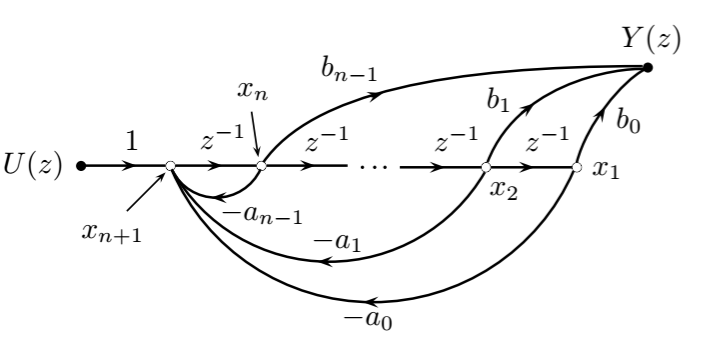
\includegraphics[width=0.73\linewidth]{Figuras/Ch14/fig5.PNG}}
\end{frame}

\begin{frame}{Forma canônica controlável - Exemplo \#01}
\begin{block}{Problema}
Considere a seguinte equação de diferenças de um sistema discreto:
$$y(k+2) = \num{1,2}y(k+1) - \num{0,2}y(k) + 10u(k+1)+5u(k)$$
Determine a forma canônica controlável deste sistema.
\end{block}
\end{frame}

\begin{frame}{Forma canônica controlável - Exemplo \#01}
\begin{block}{Resolução}
\begin{itemize}
    \item O primeiro passo é determinar a função de transferência do sistema, por meio da transformada $\mathcal{Z}$:
\end{itemize}
$$Y(z)(z^2 - \num{1,2}z + \num{0,2}) = U(z)(10z + 5) \implies \dfrac{Y(z)}{U(z)} = G(z) = \dfrac{10z + 5}{z^2 - \num{1,2}z + \num{0,2}}$$
\begin{itemize}
    \item Por inspeção: $a_1 = - \num{1,2}$; $a_0 = \num{0,2}$; $b_1 = 10$; $b_0 = 5$
    \item Deste modo, a forma canônica controlável de $G(z)$ é representada como:
\end{itemize}
\begin{align*}
    \begin{bmatrix} x_1(k+1) \\ x_2(k+1) \end{bmatrix}
    &=
    \begin{bmatrix}
    0 & 1 \\ -\num{0,2} & \num{1,2}
    \end{bmatrix}
    \begin{bmatrix}
    x_1(k) \\ x_2(k)
    \end{bmatrix}
    +
    \begin{bmatrix}
    0 \\ 1
    \end{bmatrix}
    u(k) \\
    y(k)
    &=
    \begin{bmatrix}
    5 & 10
    \end{bmatrix}
    \begin{bmatrix}
    x_1(k) \\ x_2(k)
    \end{bmatrix}
\end{align*}
\end{block}
\end{frame}

\begin{frame}{Forma canônica controlável - Exemplo \#02}
\begin{block}{Problema}
Considere o diagrama de fluxo de sinal mostrado na figura abaixo. Escreva as equações de estado e de saída para esse sistema.
\end{block}
\centerline{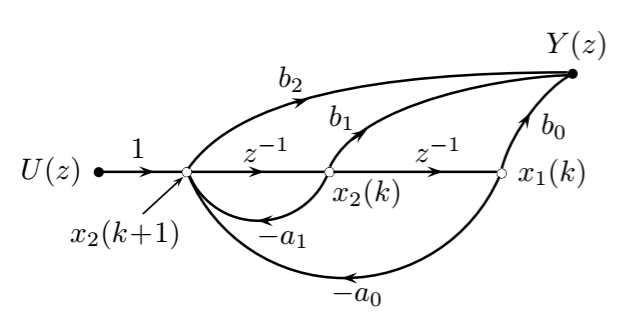
\includegraphics[width=0.73\linewidth]{Figuras/Ch14/fig6.PNG}}
\end{frame}

\begin{frame}{Forma canônica controlável - Exemplo \#02}
\begin{block}{Resolução}
\begin{itemize}
    \item As variáveis de estado são aquelas indicadas na saída dos ramos com ganho $z^{-1}$. 
    \item O nó que antecede o último ramo com ganho $z^{-1}$ tanto corresponde à variável $x_2(k)$, como corresponde a $x_1(k+1)$.
    \item Para o nó $x_2(k+1)$ temos três ramos chegando. Deste modo,
\end{itemize}

$$x_2(k+1) = -a_0 x_1(k) -a_1 x_2(k) + u(k)$$
\vspace{-0.2cm}
\begin{itemize}
    \item Para a saída $y(k)$, temos:
\end{itemize}

$$y(k) = b_0 x_1(k) + b_1 x_2(k) + b_2x_2(k+1)$$
\end{block}
\end{frame}

\begin{frame}{Forma canônica controlável - Exemplo \#02}
\begin{block}{Resolução}
\begin{itemize}
    \item A equação de saída é uma combinação linear  das variáveis de estado e, possivelmente da entrada, em que $\bm{x}(k)$ é o mesmo vetor de estado da equação dinâmica. Sendo assim, 
\end{itemize}

$$y(k) = b_0 x_1(k) + b_1 x_2(k) + b_2[-a_0 x_1(k) -a_1 x_2(k) + u(k)]$$

\begin{itemize}
    \item Deste modo, a representação em espaço de estados fica:
\end{itemize}

\begin{align*}
    \begin{bmatrix} x_1(k+1) \\ x_2(k+1) \end{bmatrix}
    &=
    \begin{bmatrix}
    0 & 1 \\ -a_0 & -a_1
    \end{bmatrix}
    \begin{bmatrix}
    x_1(k) \\ x_2(k)
    \end{bmatrix}
    +
    \begin{bmatrix}
    0 \\ 1
    \end{bmatrix}
    u(k) \\
    y(k)
    &=
    \begin{bmatrix}
    b_0-a_0b_2 & b_1-a_1b_2
    \end{bmatrix}
    \begin{bmatrix}
    x_1(k) \\ x_2(k)
    \end{bmatrix}
    + b_2 u(k) 
\end{align*}
\end{block}
\end{frame}

\begin{frame}{Forma canônica observável}
\begin{block}{Representação}
\begin{itemize}
    \item A \textbf{forma canônica observável} de $G(z)$ é representada como:
\end{itemize}

\begin{align*}
    \begin{bmatrix} x_1(k+1) \\ x_2(k+1) \\ \vdots \\  x_{n-1}(k+1) \\ x_n(k+1) \end{bmatrix}
    &=
    \begin{bmatrix}
    -a_{n-1} & 1 & 0 & \cdots & 0 \\
    -a_{n-2} & 0 & 1 & \cdots & 0 \\
     \vdots & \vdots & \vdots & \ddots & \vdots \\
    -a_1 & 0 & 0 & \cdots & 1 \\
    -a_0 & 0 & 0 & \cdots & 0
    \end{bmatrix}
    \begin{bmatrix} x_1(k) \\ x_2(k) \\ \vdots \\  x_{n-1}(k) \\ x_n(k) \end{bmatrix}
    +
    \begin{bmatrix}
    b_{n-1} \\ b_{n-2} \\ \vdots \\ b_1 \\ b_0
    \end{bmatrix}
    u(k) \\
    y(k)
    &=
    \begin{bmatrix}
    1 & 0 & \cdots & 0 & 0 
    \end{bmatrix}
    \begin{bmatrix}
    x_1(k) \\ x_2(k) \\ \vdots \\  x_{n-1}(k) \\ x_n(k)
    \end{bmatrix}
\end{align*}
\end{block}
\end{frame}

\begin{frame}{Forma canônica observável}
\begin{block}{Comentários}
\begin{itemize}
    \item A forma canônica observável também é uma \textbf{realização} (\textit{implementação}) da função de transferência $G(z)$.
    \item Dada uma função de transferência $G(z)$, a forma canônica observável pode ser obtida por \textbf{inspeção}.
    \item Além disso, todas as variáveis de estado $x_1$ e $x_n$ \textbf{aparecem na saída}, independentemente dos valores de $a_i$ e $b_j$ (\textit{o que justifica o ``observável"}).
\end{itemize}
\end{block}
\end{frame}

\begin{frame}{Forma canônica observável}
\begin{block}{Comentários}
\begin{itemize}
    \item As variáveis de estado são as saídas dos blocos com o operador de atraso $q^{-1}$ no \textbf{diagrama de simulação}. 
\end{itemize}
\end{block}
\centerline{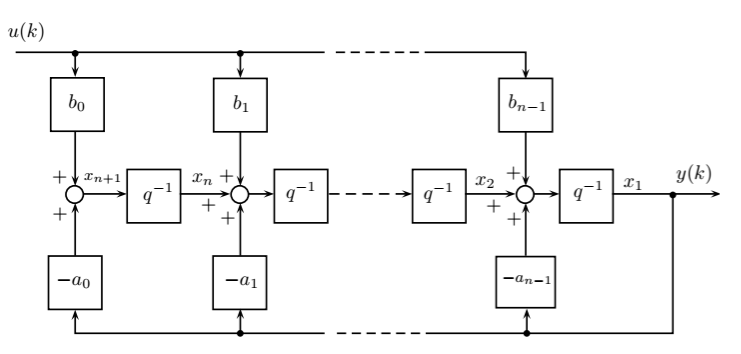
\includegraphics[width=0.8\linewidth]{Figuras/Ch14/fig7.PNG}}
\end{frame}

\begin{frame}{Forma canônica observável - Exemplo \#01}
\begin{block}{Problema}
Considere a seguinte equação de diferenças de um sistema discreto:
$$y(k+2) = \num{1,2}y(k+1) - \num{0,2}y(k) + 10u(k+1)+5u(k)$$
Determine a forma canônica observável deste sistema.
\end{block}
\end{frame}

\begin{frame}{Forma canônica observável - Exemplo \#01}
\begin{block}{Resolução}
\begin{itemize}
    \item O primeiro passo é determinar a função de transferência do sistema, por meio da transformada $\mathcal{Z}$:
\end{itemize}
$$Y(z)(z^2 - \num{1,2}z + \num{0,2}) = U(z)(10z + 5) \implies \dfrac{Y(z)}{U(z)} = G(z) = \dfrac{10z + 5}{z^2 - \num{1,2}z + \num{0,2}}$$
\begin{itemize}
    \item Por inspeção: $a_1 = - \num{1,2}$; $a_0 = \num{0,2}$; $b_1 = 10$; $b_0 = 5$
    \item Deste modo, a forma canônica observável de $G(z)$ é representada como:
\end{itemize}
\begin{align*}
    \begin{bmatrix} x_1(k+1) \\ x_2(k+1) \end{bmatrix}
    &=
    \begin{bmatrix}
    \num{1,2} & 1 \\ -\num{0,2} & 0
    \end{bmatrix}
    \begin{bmatrix}
    x_1(k) \\ x_2(k)
    \end{bmatrix}
    +
    \begin{bmatrix}
    10 \\ 5
    \end{bmatrix}
    u(k) \\
    y(k)
    &=
    \begin{bmatrix}
    1 & 0
    \end{bmatrix}
    \begin{bmatrix}
    x_1(k) \\ x_2(k)
    \end{bmatrix}
\end{align*}
\end{block}
\end{frame}

\begin{frame}{Forma canônica observável - Exemplo \#02}
\begin{block}{Problema}
	Considere a seguinte função de transferência discreta:
	$$\dfrac{Y(z)}{U(z)}= \dfrac{b_2z^2 + b_1z + b_0}{z^2 + a_1z + a_0}$$
	Determine a forma canônica observável deste sistema.
\end{block}
\end{frame}

\begin{frame}{Forma canônica observável - Exemplo \#02}
\begin{block}{Resolução}
	\begin{itemize}
		\item Como primeiro passo precisaremos realizar uma etapa da divisão polinomial. A função de transferência fica no seguinte formato:
	\end{itemize}
	$$ \dfrac{Y(z)}{U(z)} = \dfrac{(b_1 - b_2a_1)z + (b_0 - b_2a_0)}{z^2 + a_1z + a_0} + b_2$$
	\begin{itemize}
		\item Deste modo, a forma canônica observável de $G(z)$ é representada como:
	\end{itemize}
	\begin{align*}
	\begin{bmatrix} x_1(k+1) \\ x_2(k+1) \end{bmatrix}
	&=
	\begin{bmatrix}
	-a_1 & 1 \\ -a_0 & 0
	\end{bmatrix}
	\begin{bmatrix}
	x_1(k) \\ x_2(k)
	\end{bmatrix}
	+
	\begin{bmatrix}
	b_1 - b_2a_1 \\ b_0 - b_2a_0
	\end{bmatrix}
	u(k) \\
	y(k)
	&=
	\begin{bmatrix}
	1 & 0
	\end{bmatrix}
	\begin{bmatrix}
	x_1(k) \\ x_2(k)
	\end{bmatrix}
	+
	\begin{bmatrix}
	b_2
	\end{bmatrix}
	u(k)
	\end{align*}
\end{block}
\end{frame}

\begin{frame}{Forma canônica de Jordan}
\begin{block}{Introdução}
\begin{itemize}
    \item Considere que $G(z)$ (\textit{sistema completo}) possa ser representado como a \textbf{interconexão de $\bm{n}$ sistemas desacoplados} de primeira ordem. Esta representação é conhecida como a \textbf{forma canônica de Jordan}.
\end{itemize}
\end{block}
\centerline{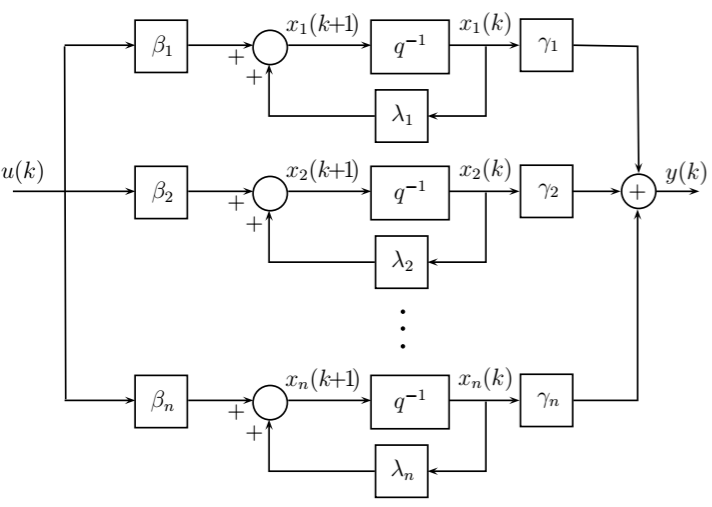
\includegraphics[width=0.65\linewidth]{Figuras/Ch14/fig8.PNG}}
\end{frame}

\begin{frame}{Forma canônica de Jordan}
\begin{block}{Representação}
\begin{itemize}
    \item A \textbf{forma canônica de Jordan} de $G(z)$ é representada como:
\end{itemize}

\begin{align*}
    \begin{bmatrix} x_1(k+1) \\ x_2(k+1) \\ \vdots \\  x_{n-1}(k+1) \\ x_n(k+1) \end{bmatrix}
    &=
    \begin{bmatrix}
    \lambda_1 & 0 & 0 & \cdots & 0 \\
    0 & \lambda_2 & 0 & \cdots & 0 \\
     \vdots & \vdots & \vdots & \ddots & \vdots \\
    0 & 0 & \cdots & \lambda_{n-1} & 0 \\
    0 & 0 & 0 & \cdots & \lambda_n
    \end{bmatrix}
    \begin{bmatrix} x_1(k) \\ x_2(k) \\ \vdots \\  x_{n-1}(k) \\ x_n(k) \end{bmatrix}
    +
    \begin{bmatrix}
    \beta_1 \\ \beta_2 \\ \vdots \\ \beta_{n-1} \\ \beta_n
    \end{bmatrix}
    u(k) \\
    y(k)
    &=
    \begin{bmatrix}
    \gamma_1 & \gamma_2 & \cdots & \gamma_{n-1} & \gamma_n
    \end{bmatrix}
    \begin{bmatrix}
    x_1(k) \\ x_2(k) \\ \vdots \\  x_{n-1}(k) \\ x_n(k)
    \end{bmatrix}
\end{align*}
\end{block}
\end{frame}

\begin{frame}{Forma canônica de Jordan}
\begin{block}{Comentários}
\begin{itemize}
    \item Cada subsistema possui a seguinte função de transferência:
\end{itemize}
$$\dfrac{Y_i(z)}{U(z)} = \dfrac{\beta_i \gamma_i}{z - \lambda_i}$$
\vspace{-0.3cm}
\begin{itemize}
    \item Desta forma, para obter a forma canônica de Jordan a partir de uma função de transferência, deve-se realizar a \textbf{decomposição em frações parciais}.
    \item Os resíduos serão $r_i = \beta_i \gamma_i$, o que mostra que a forma  canônica de Jordan, a partir de uma função  de transferência, \textbf{não é única}, pois é possível  fatorar os resíduos de infinitas formas diferentes.
\end{itemize}
\end{block}
\end{frame}

\begin{frame}{Forma canônica de Jordan - Exemplo \#01}
\begin{block}{Problema}
Considere a seguinte equação de diferenças de um sistema discreto:
$$y(k+2) = \num{1,2}y(k+1) - \num{0,2}y(k) + 10u(k+1)+5u(k)$$
Determine a forma canônica de Jordan deste sistema.
\end{block}
\end{frame}

\begin{frame}{Forma canônica de Jordan - Exemplo \#01}
\begin{block}{Resolução}
\begin{itemize}
    \item O primeiro passo é determinar a função de transferência do sistema, por meio da transformada $\mathcal{Z}$. Após isto, é necessário fazer a decomposição em frações parciais (\textit{a cargo do leitor}):
\end{itemize}
$$Y(z)(z^2 - \num{1,2}z + \num{0,2}) = U(z)(10z + 5) \implies \dfrac{Y(z)}{U(z)} = G(z) = \dfrac{10z + 5}{z^2 - \num{1,2}z + \num{0,2}}$$
$$G(z) = \dfrac{150/8}{z-1} - \dfrac{70/8}{z-\num{0,2}}$$
\vspace{-0.3cm}
\begin{itemize}
    \item Por inspeção: $\beta_1 = 150$; $\gamma_1 = 1/8$; $\lambda_1 = 1$; $\beta_2 = -70$; $\gamma_2 = 1/8$; $\lambda_2 = \num{0,2}$
    \item Deste modo, a forma canônica de Jordan de $G(z)$ é representada como:
\end{itemize}
\begin{align*}
    \begin{bmatrix} x_1(k+1) \\ x_2(k+1) \end{bmatrix}
    &=
    \begin{bmatrix}
    1 & 0 \\ 0 & \num{0,2}
    \end{bmatrix}
    \begin{bmatrix}
    x_1(k) \\ x_2(k)
    \end{bmatrix}
    +
    \begin{bmatrix}
    150 \\ -70
    \end{bmatrix}
    u(k) \\
    y(k)
    &=
    \begin{bmatrix}
    1/8 & 1/8
    \end{bmatrix}
    \begin{bmatrix}
    x_1(k) \\ x_2(k)
    \end{bmatrix}
\end{align*}
\end{block}
\end{frame}

\begin{frame}{Matriz de transferência}
\begin{block}{Introdução}
\begin{itemize}
    \item As três formas canônicas vistas anteriormente permitem representar um sistema em espaço de estados a partir de uma função de transferência.
    \item Podemos ainda \textbf{encontrar a matriz de transferência} (\textit{função de transferência para sistemas SISO}) a partir de qualquer representação em espaço de estados.
\end{itemize}
\end{block}
\end{frame}

\begin{frame}{Matriz de transferência}
\begin{block}{Formulação matemática}
Seja a representação padrão de um SLIT em espaço de estados:
\begin{align*}
    \bm{x}(k+1) &= A\bm{x}(k) + B\bm{u}(k) \\
    \bm{y}(k) &= C\bm{x}(k) + D\bm{u}(k)
\end{align*}
A transformada $\mathcal{Z}$, considerando condições iniciais nulas, é:
\begin{align*}
    zX(z) &= AX(z) + BU(z) \\
    Y(z)  &= CX(z) + DU(z)
\end{align*}
Podemos reescrever a equação dinâmica como
$$(zI - A)X(z) = BU(z) \implies X(z) = (zI - A)^{-1}BU(z)$$
Substituindo na equação de saída, temos:
$$Y(z) = C(zI - A)^{-1} BU(z) + DU(z)$$
\end{block}
\end{frame}

\begin{frame}{Matriz de transferência}
\begin{block}{Formulação matemática}
Desta forma,
$$\boxed{G(z) = C(zI - A)^{-1} B + D}$$
que é a \textbf{matriz de transferência} que tem dimensão $p \times r$.
\begin{itemize}
    \item No caso de sistemas SISO ($r=1$ e $p=1$), $G(z)$ é uma \textbf{função de transferência}. 
    \item Se o sistema tiver mais de uma entrada e/ou mais de uma saída, cada elemento da matriz de transferência $G(z)$ é uma função de transferência que descreve como uma determinada entrada é ``transferida” para a saída em questão. 
\end{itemize}
\end{block}
\end{frame}

\begin{frame}{Matriz de transferência - Exemplo \#01}
\begin{block}{Problema}
Considere a seguinte representação em espaço de estados na forma canônica controlável:
\begin{align*}
    \begin{bmatrix} x_1(k+1) \\ x_2(k+1) \end{bmatrix}
    &=
    \begin{bmatrix}
    0 & 1 \\ -\num{0,2} & \num{1,2}
    \end{bmatrix}
    \begin{bmatrix}
    x_1(k) \\ x_2(k)
    \end{bmatrix}
    +
    \begin{bmatrix}
    0 \\ 1
    \end{bmatrix}
    u(k) \\
    y(k)
    &=
    \begin{bmatrix}
    5 & 10
    \end{bmatrix}
    \begin{bmatrix}
    x_1(k) \\ x_2(k)
    \end{bmatrix}
\end{align*}
Determine a função de transferência deste sistema.
\end{block}
\end{frame}

\begin{frame}{Matriz de transferência - Exemplo \#01}
\begin{block}{Resolução}
\begin{itemize}
    \item Realizando os devidos cálculos, temos:
\end{itemize}
\begin{align*}
    G(z) &= C(zI - A)^{-1} B + D \\
    &= \begin{bmatrix}
    5 & 10
    \end{bmatrix}
    \begin{bmatrix}
    z & -1 \\ \num{0,2} & z-\num{1,2}
    \end{bmatrix}^{-1} 
    \begin{bmatrix}
    0 \\ 1
    \end{bmatrix}
    + 0 \\
    &= \dfrac{1}{z^2-\num{1,2}z+\num{0,2}}
    \begin{bmatrix}
    5 & 10
    \end{bmatrix}
    \begin{bmatrix}
    z-\num{1,2} & 1 \\ -\num{0,2} & z
    \end{bmatrix}
    \begin{bmatrix}
    0 \\ 1
    \end{bmatrix} \\
    &= \dfrac{1}{z^2-\num{1,2}z+\num{0,2}}
    \begin{bmatrix}
    5 & 10
    \end{bmatrix}
    \begin{bmatrix}
    1 \\ z
    \end{bmatrix} \\
    &= \dfrac{10z+5}{z^2-\num{1,2}z+\num{0,2}}
\end{align*}
\vspace{-0.3cm}
\begin{itemize}
    \item[] que é o exemplo \textit{dual} feito anteriormente.
\end{itemize}
\end{block}
\end{frame}

\cprotect\frame{
\frametitle{\MATLAB}
\begin{block}{}
\begin{verbatim}
>>[num,den]=ss2tf(A,B,C,D) 
\end{verbatim}
converte um sistema dinâmico representado em espaço de estados $\bm{(A,B,C,D)}$ em sua respectiva função de transferência \textbf{[num, den]}. \\
\vspace{0.2cm}
\textbf{Exemplo}: conversão do exemplo \#01
\end{block}
\centerline{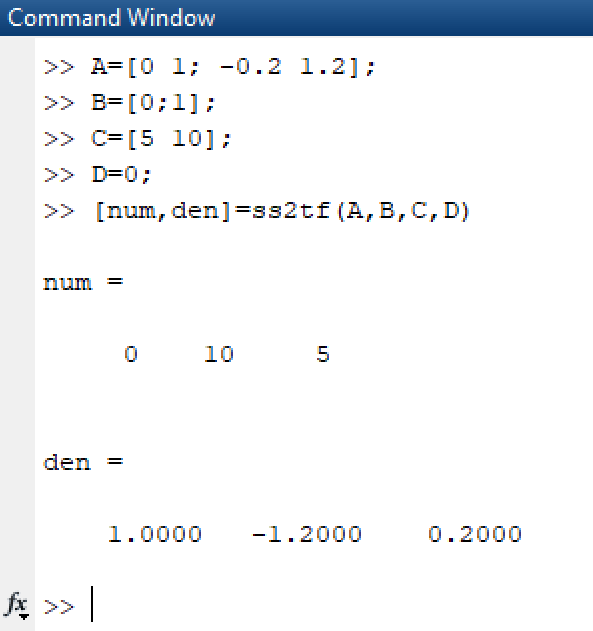
\includegraphics[width=0.4\linewidth]{Figuras/Ch14/fig9.PNG}}
}

\begin{frame}{Matriz de transferência - Exemplo \#02}
\begin{block}{Problema}
Considere a seguinte representação em espaço de estados na forma canônica observável:
\begin{align*}
    \begin{bmatrix} x_1(k+1) \\ x_2(k+1) \end{bmatrix}
    &=
    \begin{bmatrix}
    \num{1,2} & 1 \\ -\num{0,2} & 0
    \end{bmatrix}
    \begin{bmatrix}
    x_1(k) \\ x_2(k)
    \end{bmatrix}
    +
    \begin{bmatrix}
    10 \\ 5
    \end{bmatrix}
    u(k) \\
    y(k)
    &=
    \begin{bmatrix}
    1 & 0
    \end{bmatrix}
    \begin{bmatrix}
    x_1(k) \\ x_2(k)
    \end{bmatrix}
\end{align*}
Determine a função de transferência deste sistema.
\end{block}
\end{frame}

\begin{frame}{Matriz de transferência - Exemplo \#02}
\begin{block}{Resolução}
\begin{itemize}
    \item Realizando os devidos cálculos, temos:
\end{itemize}
\begin{align*}
    G(z) &= C(zI - A)^{-1} B + D \\
    &= \begin{bmatrix}
    1 & 0
    \end{bmatrix}
    \begin{bmatrix}
    z-\num{1,2} & -1 \\ \num{0,2} & z
    \end{bmatrix}^{-1} 
    \begin{bmatrix}
    10 \\ 5
    \end{bmatrix}
    + 0 \\
    &= \dfrac{1}{z^2-\num{1,2}z+\num{0,2}}
    \begin{bmatrix}
    1 & 0
    \end{bmatrix}
    \begin{bmatrix}
    z & 1 \\ -\num{0,2} & z-\num{1,2}
    \end{bmatrix}
    \begin{bmatrix}
    10 \\ 5
    \end{bmatrix} \\
    &= \dfrac{1}{z^2-\num{1,2}z+\num{0,2}}
    \begin{bmatrix}
    1 & 0
    \end{bmatrix}
    \begin{bmatrix}
    10z+5 \\ 5z-8
    \end{bmatrix} \\
    &= \dfrac{10z+5}{z^2-\num{1,2}z+\num{0,2}}
\end{align*}
\vspace{-0.3cm}
\begin{itemize}
    \item[] que é o exemplo \textit{dual} feito anteriormente.
\end{itemize}
\end{block}
\end{frame}

\cprotect\frame{
\frametitle{\MATLAB}
\begin{block}{}
\begin{verbatim}
>>[num,den]=ss2tf(A,B,C,D) 
\end{verbatim}
converte um sistema dinâmico representado em espaço de estados $\bm{(A,B,C,D)}$ em sua respectiva função de transferência \textbf{[num, den]}. \\
\vspace{0.2cm}
\textbf{Exemplo}: conversão do exemplo \#02
\end{block}
\centerline{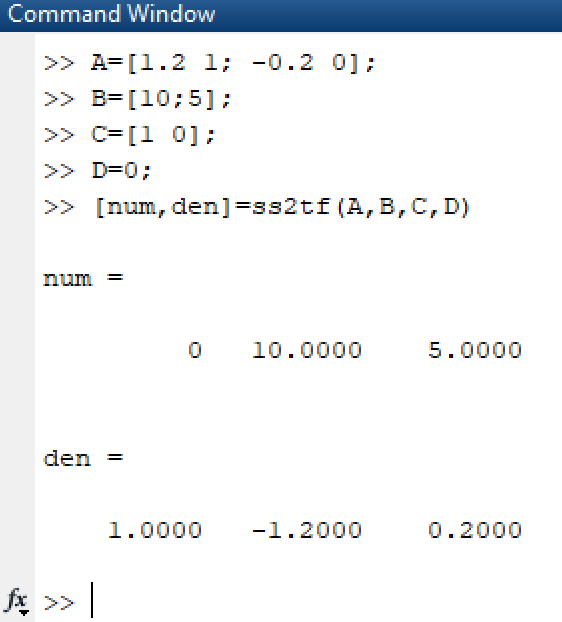
\includegraphics[width=0.38\linewidth]{Figuras/Ch14/fig10.PNG}}
}

































\begin{frame}{Matriz de transferência - Exemplo \#03}
\begin{block}{Problema}
Considere a seguinte representação em espaço de estados na forma canônica de Jordan:
\begin{align*}
    \begin{bmatrix} x_1(k+1) \\ x_2(k+1) \end{bmatrix}
    &=
    \begin{bmatrix}
    1 & 0 \\ 0 & \num{0,2}
    \end{bmatrix}
    \begin{bmatrix}
    x_1(k) \\ x_2(k)
    \end{bmatrix}
    +
    \begin{bmatrix}
    150 \\ -70
    \end{bmatrix}
    u(k) \\
    y(k)
    &=
    \begin{bmatrix}
    1/8 & 1/8
    \end{bmatrix}
    \begin{bmatrix}
    x_1(k) \\ x_2(k)
    \end{bmatrix}
\end{align*}
Determine a função de transferência deste sistema.
\end{block}
\end{frame}

\begin{frame}{Matriz de transferência - Exemplo \#03}
\begin{block}{Resolução}
\begin{itemize}
    \item Realizando os devidos cálculos, temos:
\end{itemize}
\begin{align*}
    G(z) &= C(zI - A)^{-1} B + D \\
    &= \begin{bmatrix}
    1/8 & 1/8
    \end{bmatrix}
    \begin{bmatrix}
    z-1 & 0 \\ 0 & z-\num{0,2}
    \end{bmatrix}^{-1} 
    \begin{bmatrix}
    150 \\ -70
    \end{bmatrix}
    + 0 \\
    &= \dfrac{1}{z^2-\num{1,2}z+\num{0,2}}
    \begin{bmatrix}
    1/8 & 1/8
    \end{bmatrix}
    \begin{bmatrix}
    z-\num{0,2} & 0 \\ 0 & z-1
    \end{bmatrix}
    \begin{bmatrix}
    150 \\ -70
    \end{bmatrix} \\
    &= \dfrac{1}{z^2-\num{1,2}z+\num{0,2}}
    \begin{bmatrix}
    1/8 & 1/8
    \end{bmatrix}
    \begin{bmatrix}
    150z-30 \\ -70z+70
    \end{bmatrix} \\
    &= \dfrac{10z+5}{z^2-\num{1,2}z+\num{0,2}}
\end{align*}
\vspace{-0.3cm}
\begin{itemize}
    \item[] que é o exemplo \textit{dual} feito anteriormente.
\end{itemize}
\end{block}
\end{frame}

\cprotect\frame{
\frametitle{\MATLAB}
\begin{block}{}
\begin{verbatim}
>>[num,den]=ss2tf(A,B,C,D) 
\end{verbatim}
converte um sistema dinâmico representado em espaço de estados $\bm{(A,B,C,D)}$ em sua respectiva função de transferência \textbf{[num, den]}. \\
\vspace{0.2cm}
\textbf{Exemplo}: conversão do exemplo \#03
\end{block}
\centerline{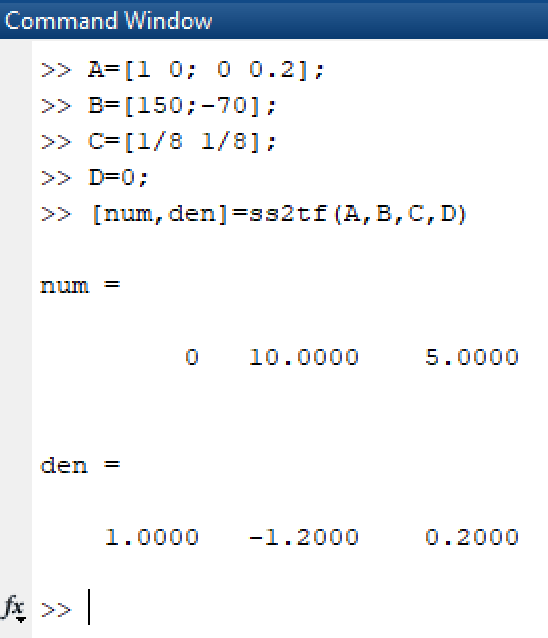
\includegraphics[width=0.36\linewidth]{Figuras/Ch14/fig11.PNG}}
}

\frame{
\frametitle{Exercícios}
\begin{block}{}
01. ``Todo polo da função de transferência também é um autovalor de $A$, mas um autovalor de $A$ pode não ser um polo da função de transferência, se este for cancelado  por um zero." Verifique esta afirmação com a seguinte função de transferência:
$$\dfrac{Y(z)}{U(z)} = \dfrac{-25z+5}{z^2-\num{1,2}z+\num{0,2}}$$
\end{block}
}

\frame{
\frametitle{Exercícios}
\begin{block}{}
02. Considere um sistema discreto representado pelo seguinte espaço de estados:
\begin{align*}
    \bm{x}(k+1) &= \begin{bmatrix}
    0 & 1 \\
    -2 & 3 \\
    \end{bmatrix}\bm{x}(k) +  \begin{bmatrix}
    0 \\
    1 \\  
    \end{bmatrix}\bm{u}(k) \\
    \bm{y}(k) &= \begin{bmatrix}
    0 & 1
    \end{bmatrix}\bm{x}(k) 
\end{align*}
    
\begin{enumerate}
    \item[(a)] Determine a função de transferência deste sistema.
    \item[(b)] Analise a estabilidade deste sistema.
    \item[(c)] Em que forma canônica está o sistema discreto em espaço de estados da questão?
\end{enumerate}
\end{block}
}

\frame{
\frametitle{Referências e exercícios complementares}
\begin{itemize}
\item AGUIRRE, Luis A. Controle de Sistemas Amostrados, 1 ed. [s.n.], 2019.
\end{itemize}
\centering{\alert{Página 286 - \textbf{Capítulo 7}}} \\
\vspace{0.4cm}
\begin{itemize}
\item FRANKLIN, Gene F.; POWELL, J. David; WOLKMAN, Michael L. Digital Control of Dynamic Systems, 3 ed. Addison-Wesley, 1998.
\end{itemize}
\centering{\alert{Página 149 - \textbf{Capítulo 4}}} \\
}